\documentclass[aspectratio=169]{beamer}

% Theme and Color Setup
\usetheme{Madrid}
\usecolortheme{whale}
\useinnertheme{rectangles}
\useoutertheme{miniframes}

% Additional Packages
\usepackage[utf8]{inputenc}
\usepackage[T1]{fontenc}
\usepackage{graphicx}
\usepackage{booktabs}
\usepackage{listings}
\usepackage{amsmath}
\usepackage{amssymb}
\usepackage{xcolor}
\usepackage{tikz}
\usepackage{pgfplots}
\pgfplotsset{compat=1.18}
\usetikzlibrary{positioning}
\usepackage{hyperref}

% Custom Colors
\definecolor{myblue}{RGB}{31, 73, 125}
\definecolor{mygray}{RGB}{100, 100, 100}
\definecolor{mygreen}{RGB}{0, 128, 0}
\definecolor{myorange}{RGB}{230, 126, 34}
\definecolor{mycodebackground}{RGB}{245, 245, 245}

% Set Theme Colors
\setbeamercolor{structure}{fg=myblue}
\setbeamercolor{frametitle}{fg=white, bg=myblue}
\setbeamercolor{title}{fg=myblue}
\setbeamercolor{section in toc}{fg=myblue}
\setbeamercolor{item projected}{fg=white, bg=myblue}
\setbeamercolor{block title}{bg=myblue!20, fg=myblue}
\setbeamercolor{block body}{bg=myblue!10}
\setbeamercolor{alerted text}{fg=myorange}

% Set Fonts
\setbeamerfont{title}{size=\Large, series=\bfseries}
\setbeamerfont{frametitle}{size=\large, series=\bfseries}
\setbeamerfont{caption}{size=\small}
\setbeamerfont{footnote}{size=\tiny}

% Code Listing Style
\lstdefinestyle{customcode}{
  backgroundcolor=\color{mycodebackground},
  basicstyle=\footnotesize\ttfamily,
  breakatwhitespace=false,
  breaklines=true,
  commentstyle=\color{mygreen}\itshape,
  keywordstyle=\color{blue}\bfseries,
  stringstyle=\color{myorange},
  numbers=left,
  numbersep=8pt,
  numberstyle=\tiny\color{mygray},
  frame=single,
  framesep=5pt,
  rulecolor=\color{mygray},
  showspaces=false,
  showstringspaces=false,
  showtabs=false,
  tabsize=2,
  captionpos=b
}
\lstset{style=customcode}

% Custom Commands
\newcommand{\hilight}[1]{\colorbox{myorange!30}{#1}}
\newcommand{\source}[1]{\vspace{0.2cm}\hfill{\tiny\textcolor{mygray}{Source: #1}}}
\newcommand{\concept}[1]{\textcolor{myblue}{\textbf{#1}}}
\newcommand{\separator}{\begin{center}\rule{0.5\linewidth}{0.5pt}\end{center}}

% Footer and Navigation Setup
\setbeamertemplate{footline}{
  \leavevmode%
  \hbox{%
  \begin{beamercolorbox}[wd=.3\paperwidth,ht=2.25ex,dp=1ex,center]{author in head/foot}%
    \usebeamerfont{author in head/foot}\insertshortauthor
  \end{beamercolorbox}%
  \begin{beamercolorbox}[wd=.5\paperwidth,ht=2.25ex,dp=1ex,center]{title in head/foot}%
    \usebeamerfont{title in head/foot}\insertshorttitle
  \end{beamercolorbox}%
  \begin{beamercolorbox}[wd=.2\paperwidth,ht=2.25ex,dp=1ex,center]{date in head/foot}%
    \usebeamerfont{date in head/foot}
    \insertframenumber{} / \inserttotalframenumber
  \end{beamercolorbox}}%
  \vskip0pt%
}

% Turn off navigation symbols
\setbeamertemplate{navigation symbols}{}

% Title Page Information
\title[Week 2: Machine Learning Basics]{Week 2: Machine Learning Basics}
\author[J. Smith]{John Smith, Ph.D.}
\institute[University Name]{Department of Computer Science\\University Name\\\vspace{0.3cm}Email: email@university.edu\\Website: www.university.edu}
\date{\today}

% Document Start
\begin{document}

\frame{\titlepage}

\begin{frame}[fragile]
    \frametitle{Introduction to Machine Learning}
    \begin{block}{What is Machine Learning?}
        Machine Learning (ML) is a subfield of Artificial Intelligence (AI) that focuses on developing algorithms and statistical models that enable computer systems to perform tasks without explicit instructions. Instead, these systems learn from and make predictions or decisions based on data.
    \end{block}
\end{frame}

\begin{frame}[fragile]
    \frametitle{Significance of Machine Learning in AI}
    \begin{enumerate}
        \item \textbf{Data-Driven Intelligence:}
        \begin{itemize}
            \item ML enables computers to analyze vast amounts of data and identify patterns that humans might overlook.
        \end{itemize}
        
        \item \textbf{Automation of Tasks:}
        \begin{itemize}
            \item Enhances productivity and efficiency across various sectors such as healthcare, finance, and transportation.
        \end{itemize}

        \item \textbf{Improved Decision Making:}
        \begin{itemize}
            \item Assists in making data-driven decisions leading to better outcomes.
        \end{itemize}

        \item \textbf{Personalization:}
        \begin{itemize}
            \item Businesses leverage ML to tailor services and enhance customer satisfaction.
        \end{itemize}
    \end{enumerate}
\end{frame}

\begin{frame}[fragile]
    \frametitle{Key Points and Example}
    \begin{block}{Key Points to Emphasize}
        \begin{itemize}
            \item \textbf{Adaptability:} ML models can adapt as new data arrives.
            \item \textbf{Challenges:} Issues include the need for quality data, model transparency, and ethical implications such as bias.
        \end{itemize}
    \end{block}
    
    \begin{block}{Example: Image Recognition}
        \begin{itemize}
            \item \textbf{Scenario:} Teaching a program to identify cats in photos.
            \item \textbf{Process:}
            \begin{enumerate}
                \item Training Data: A dataset of labeled images (some with cats, some without).
                \item Learning: The ML model analyzes the features of the images.
                \item Prediction: Identifying whether new images contain a cat.
            \end{enumerate}
        \end{itemize}
    \end{block}
\end{frame}

\begin{frame}[fragile]
    \frametitle{Conclusion}
    Machine Learning is revolutionizing technology and society by enabling systems to learn from data and enhance functionality. Understanding its foundations is essential for anyone looking to work in AI, data science, or related fields.
\end{frame}

\begin{frame}[fragile]
    \frametitle{What is Machine Learning? - Definition}
    \begin{block}{Definition of Machine Learning}
        Machine Learning (ML) is a subset of artificial intelligence (AI) that enables systems to learn and make decisions from data without being explicitly programmed.
    \end{block}
    \begin{itemize}
        \item ML algorithms identify patterns within the data.
        \item These patterns are used to perform tasks such as making predictions or classifying information.
    \end{itemize}
\end{frame}

\begin{frame}[fragile]
    \frametitle{What is Machine Learning? - Differences from Traditional Programming}
    \begin{block}{Traditional Programming versus Machine Learning}
        \begin{enumerate}
            \item \textbf{Programming Approach}
                \begin{itemize}
                    \item Traditional Programming: Developers write explicit rules to solve problems.
                    \item Machine Learning: Models learn from data without explicit rules.
                \end{itemize}
            \item \textbf{Example}
                \begin{itemize}
                    \item Traditional: Specific rules to identify spam emails, e.g., "If 'free' is in the email, classify as spam."
                    \item ML: Algorithms analyze a dataset of labeled emails to uncover patterns.
                \end{itemize}
            \item \textbf{Output}
                \begin{itemize}
                    \item Traditional: Predictable outputs based on rules.
                    \item ML: Outputs vary based on the model's understanding of trained data.
                \end{itemize}
        \end{enumerate}
    \end{block}
\end{frame}

\begin{frame}[fragile]
    \frametitle{What is Machine Learning? - Key Points and Conclusion}
    \begin{block}{Key Points to Emphasize}
        \begin{itemize}
            \item ML models improve performance with more data.
            \item They adapt to new data, making them useful in dynamic environments.
            \item Applications include recommendation systems (Netflix, Amazon) and predictive analytics (finance).
        \end{itemize}
    \end{block}
    \begin{block}{Conclusion}
        Understanding the difference between traditional programming and machine learning is fundamental in grasping how machines learn from data, marking a major advancement in computer science and AI.
    \end{block}
\end{frame}

\begin{frame}[fragile]
    \frametitle{Types of Machine Learning - Introduction}
    Machine Learning (ML) can be categorized into three primary types based on how learning occurs from the provided data. Understanding these types is crucial for selecting the appropriate ML approach for different problems.
\end{frame}

\begin{frame}[fragile]
    \frametitle{Types of Machine Learning - 1. Supervised Learning}
    \begin{block}{Definition}
        Supervised learning involves training a model on a labeled dataset, meaning that each training example is paired with an output label.
    \end{block}
    
    \begin{block}{How It Works}
        The algorithm learns to map inputs to desired outputs by minimizing the error between predicted and actual outputs.
    \end{block}

    \begin{block}{Example}
        Image Classification: Given a dataset of images of cats and dogs labeled as 'cat' or 'dog', the model learns to identify and classify new images based on learned features.
    \end{block}

    \begin{itemize}
        \item Requires labeled data.
        \item Common algorithms: Linear Regression, Decision Trees, SVM.
    \end{itemize}
\end{frame}

\begin{frame}[fragile]
    \frametitle{Types of Machine Learning - 1. Supervised Learning (Code Example)}
    \begin{lstlisting}[language=Python]
from sklearn.model_selection import train_test_split
from sklearn.ensemble import RandomForestClassifier

# Sample dataset
X, y = load_data()  # feature data and labels
X_train, X_test, y_train, y_test = train_test_split(X, y, test_size=0.2)

# Model training
model = RandomForestClassifier()
model.fit(X_train, y_train)
    \end{lstlisting}
\end{frame}

\begin{frame}[fragile]
    \frametitle{Types of Machine Learning - 2. Unsupervised Learning}
    \begin{block}{Definition}
        Unsupervised learning deals with datasets that do not have labeled outputs. The goal is to infer the natural structure present within a set of data points.
    \end{block}

    \begin{block}{How It Works}
        The algorithm identifies patterns, clusters, or associations in the data without predefined labels.
    \end{block}

    \begin{block}{Example}
        Customer Segmentation: Analyzing purchasing behavior data to identify distinct groups of customers based on their buying habits.
    \end{block}

    \begin{itemize}
        \item Suitable for exploratory data analysis.
        \item Common algorithms: K-Means, Hierarchical Clustering, PCA.
    \end{itemize}

    % Add a diagram placeholder here as needed
\end{frame}

\begin{frame}[fragile]
    \frametitle{Types of Machine Learning - 3. Reinforcement Learning}
    \begin{block}{Definition}
        Reinforcement learning involves training an agent to make decisions by taking actions in an environment to maximize cumulative reward. It is inspired by behavioral psychology.
    \end{block}

    \begin{block}{How It Works}
        The agent learns through trial and error, receiving feedback in the form of rewards or penalties, which influences future actions.
    \end{block}

    \begin{block}{Example}
        Game Playing: Training an AI to play chess, where it learns strategies based on winning or losing games.
    \end{block}

    \begin{itemize}
        \item Agent-interaction with an environment.
        \item Key concepts: reward signals, policy, and value functions.
    \end{itemize}

    % Add a flowchart placeholder here as needed
\end{frame}

\begin{frame}[fragile]
    \frametitle{Types of Machine Learning - Summary}
    \begin{itemize}
        \item \textbf{Supervised Learning}: Uses labeled data to predict outcomes. Examples include classification and regression.
        \item \textbf{Unsupervised Learning}: Deals with unlabeled data to find hidden patterns. Examples include clustering and association.
        \item \textbf{Reinforcement Learning}: An agent learns to make decisions based on rewards and penalties through its interactions with the environment.
    \end{itemize}
    
    Understanding these types of machine learning paves the way for implementing effective models tailored to specific problem domains!
\end{frame}

\begin{frame}[fragile]
    \frametitle{Key Concepts in Machine Learning - Introduction}
    \begin{block}{Definition}
        Machine learning is a core subfield of artificial intelligence that focuses on building systems that learn from data to improve their performance over time. 
    \end{block}
    \begin{block}{Overview}
        In this presentation, we will explore fundamental concepts that form the foundation of machine learning.
    \end{block}
\end{frame}

\begin{frame}[fragile]
    \frametitle{Key Concepts in Machine Learning - Models}
    \begin{itemize}
        \item \textbf{Definition}: A model is a mathematical representation that outputs predictions or classifications based on the input data.
        \item \textbf{Example}: A linear regression model might predict house prices based on features like size, location, and age.
    \end{itemize}
\end{frame}

\begin{frame}[fragile]
    \frametitle{Key Concepts in Machine Learning - Training Data}
    \begin{itemize}
        \item \textbf{Definition}: This is the dataset used to train a machine learning model, allowing it to learn and make predictions.
        \item \textbf{Example}: For an image classifier, the training data might consist of thousands of labeled images (e.g., cats and dogs).
    \end{itemize}
\end{frame}

\begin{frame}[fragile]
    \frametitle{Key Concepts in Machine Learning - Features}
    \begin{itemize}
        \item \textbf{Definition}: Features are the individual measurable properties or characteristics of the data used by the model.
        \item \textbf{Example}: For a car price prediction model, features could include make, model, year, mileage, and color.
    \end{itemize}
\end{frame}

\begin{frame}[fragile]
    \frametitle{Key Concepts in Machine Learning - Labels}
    \begin{itemize}
        \item \textbf{Definition}: Labels are the target outcomes that we want to predict, guiding the learning process.
        \item \textbf{Example}: In a dataset for classifying emails, the label would be either "spam" or "not spam."
    \end{itemize}
\end{frame}

\begin{frame}[fragile]
    \frametitle{Key Concepts in Machine Learning - Key Points}
    \begin{itemize}
        \item Models learn from training data by recognizing patterns between features and labels.
        \item The quality and quantity of training data significantly influence model performance.
        \item Selecting relevant features is critical; irrelevant features can lead to overfitting.
    \end{itemize}
\end{frame}

\begin{frame}[fragile]
    \frametitle{Key Concepts in Machine Learning - Visual Representation}
    \begin{center}
        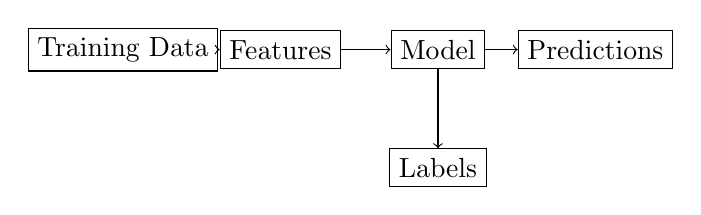
\begin{tikzpicture}
            \node (data) at (0,0) [draw] {Training Data};
            \node (features) at (2,0) [draw] {Features};
            \node (model) at (4,0) [draw] {Model};
            \node (predictions) at (6,0) [draw] {Predictions};
            \node (labels) at (4,-1.5) [draw] {Labels};

            \draw[->] (data) -- (features);
            \draw[->] (features) -- (model);
            \draw[->] (model) -- (predictions);
            \draw[<-] (labels) -- (model);
        \end{tikzpicture}
    \end{center}
\end{frame}

\begin{frame}[fragile]
    \frametitle{Key Concepts in Machine Learning - Conclusion}
    \begin{block}{Summary}
        Understanding the basic concepts—models, training data, features, and labels—is essential for anyone looking to start in machine learning. 
    \end{block}
    \begin{block}{Significance}
        These elements work together to create systems that learn from experience, making informed predictions based on new data inputs.
    \end{block}
\end{frame}

\begin{frame}[fragile]
    \frametitle{Key Concepts in Machine Learning - Next Steps}
    \begin{block}{Exploration}
        In the following slide, we will introduce TensorFlow, a powerful framework for building and deploying machine learning models.
    \end{block}
    \begin{block}{Invitation}
        Feel free to dive deeper into each concept and explore their interconnections throughout your machine learning journey!
    \end{block}
\end{frame}

\begin{frame}[fragile]
    \frametitle{What is TensorFlow?}
    \begin{itemize}
        \item \textbf{Definition}: TensorFlow is an open-source machine learning framework developed by Google Brain. It is designed for building, training, and deploying machine learning models with a focus on deep learning, neural networks, and numerical computation.
    \end{itemize}
\end{frame}

\begin{frame}[fragile]
    \frametitle{Key Features of TensorFlow}
    \begin{enumerate}
        \item \textbf{Scalability}:
        \begin{itemize}
            \item Handles tasks from small-scale projects to large-scale distributed machine learning, suitable for both researchers and enterprises.
        \end{itemize}
        
        \item \textbf{Versatility}:
        \begin{itemize}
            \item Supports multiple languages: Python, JavaScript, C++, and more.
            \item Compatible with desktops, servers, mobile devices, and cloud environments.
        \end{itemize}
        
        \item \textbf{Ecosystem}:
        \begin{itemize}
            \item Includes TensorBoard (for visualization), TensorFlow Lite (for mobile/embedded devices), and TensorFlow Extended (for production ML pipelines).
        \end{itemize}
    \end{enumerate}
\end{frame}

\begin{frame}[fragile]
    \frametitle{Basic Concepts}
    \begin{itemize}
        \item \textbf{Tensors}: Fundamental data structure in TensorFlow, represented as multi-dimensional arrays.
        \begin{block}{Examples}
            \begin{lstlisting}[language=Python]
            import tensorflow as tf
            
            # Creating a tensor
            scalar = tf.constant(7)   # 0D tensor
            vector = tf.constant([1, 2, 3])  # 1D tensor
            matrix = tf.constant([[1, 2], [3, 4]])  # 2D tensor
            \end{lstlisting}
            \end{block}
        
        \item \textbf{Computational Graphs}: TensorFlow uses a data flow graph to represent computation. Each node represents an operation (like addition/multiplication), and edges represent tensors flowing between those operations.
    \end{itemize}
\end{frame}

\begin{frame}[fragile]
    \frametitle{Example of Use}
    \begin{itemize}
        \item \textbf{Building a Simple Model}:
        \begin{block}{Linear Regression Model}
            \begin{lstlisting}[language=Python]
            import tensorflow as tf
            
            # Define the model
            model = tf.keras.Sequential([
                tf.keras.layers.Dense(units=1, input_shape=[1])
            ])

            model.compile(optimizer='sgd', loss='mean_squared_error')

            # Sample data
            xs = [1, 2, 3, 4]
            ys = [2, 4, 6, 8]

            # Train the model
            model.fit(xs, ys, epochs=500)
            \end{lstlisting}
            \end{block}
    \end{itemize}
\end{frame}

\begin{frame}[fragile]
    \frametitle{Key Points to Emphasize}
    \begin{itemize}
        \item \textbf{Community Support}: TensorFlow has a vast community and extensive documentation, making it easier for both beginners and professionals to find resources and solutions.
        \item \textbf{Integration with Other Tools}: TensorFlow works seamlessly with libraries like Keras, enhancing usability for developing neural networks.
    \end{itemize}
\end{frame}

\begin{frame}[fragile]
    \frametitle{Conclusion}
    \begin{itemize}
        \item TensorFlow is a powerful tool at the forefront of machine learning and deep learning research and production.
        \item Understanding its foundational concepts is crucial for anyone looking to delve into machine learning.
    \end{itemize}
\end{frame}

\begin{frame}[fragile]
    \frametitle{Why Use TensorFlow? - Introduction}
    TensorFlow is an open-source machine learning framework developed by Google. It provides an extensive ecosystem for building and deploying machine learning models, making it a popular choice among data scientists and developers.
\end{frame}

\begin{frame}[fragile]
    \frametitle{Why Use TensorFlow? - Key Benefits}
    \begin{enumerate}
        \item \textbf{Flexibility}
        \begin{itemize}
            \item Supports various programming paradigms, including imperative and declarative programming styles.
            \item Example: Users can build custom model architectures using the TensorFlow Keras API.
        \end{itemize}
        
        \item \textbf{Scalability}
        \begin{itemize}
            \item Designed to scale seamlessly across multiple CPUs and GPUs.
            \item Example: Handles large datasets and employs distributed computing for faster processing.
        \end{itemize}
        
        \item \textbf{Robust Ecosystem}
        \begin{itemize}
            \item Rich set of libraries and tools, such as TensorBoard for visualization and TensorFlow Extended (TFX) for production pipelines.
            \item Example: TensorBoard visualizes model training metrics for better hyperparameter tuning.
        \end{itemize}
    \end{enumerate}
\end{frame}

\begin{frame}[fragile]
    \frametitle{Why Use TensorFlow? - Key Benefits (cont.)}
    \begin{enumerate}
        \setcounter{enumi}{3} % Continue enumerating
        \item \textbf{Support for Multiple Languages}
        \begin{itemize}
            \item APIs available for popular languages such as Python, C++, and JavaScript.
            \item \begin{lstlisting}[language=Python]
import tensorflow as tf
model = tf.keras.models.Sequential([
    tf.keras.layers.Dense(128, activation='relu', input_shape=(input_dim,)),
    tf.keras.layers.Dense(output_dim, activation='softmax')
])
            \end{lstlisting}
        \end{itemize}

        \item \textbf{Community and Resources}
        \begin{itemize}
            \item Large community contributing to development with extensive resources, tutorials, and pre-trained models.
            \item Example: The TensorFlow Model Garden offers state-of-the-art pre-trained models.
        \end{itemize}

        \item \textbf{Support for Advanced Techniques}
        \begin{itemize}
            \item Functionality for advanced techniques including neural networks and reinforcement learning.
            \item Example: Illustrations of neural network architectures showcasing data flow.
        \end{itemize}
    \end{enumerate}
\end{frame}

\begin{frame}[fragile]
    \frametitle{Why Use TensorFlow? - Conclusion}
    With its flexibility, scalability, robust ecosystem, and strong community support, TensorFlow stands out as one of the premier frameworks for machine learning. Whether you're a beginner or an experienced developer, TensorFlow provides the tools you need to innovate and push the boundaries of what is possible with machine learning.

    \textbf{Key Points to Emphasize:}
    \begin{itemize}
        \item Flexibility and scalability suitable for projects of any size.
        \item Extensive libraries and tools enhance productivity.
        \item Strong community and resources support users in their learning journey.
    \end{itemize}

    Feel free to ask any questions or explore more about how TensorFlow can meet your machine learning needs!
\end{frame}

\begin{frame}[fragile]
    \frametitle{Setting Up the Environment for TensorFlow}
    \begin{block}{Introduction}
        Setting up a proper development environment is crucial for your machine learning projects. 
        In this slide, we will guide you through the steps needed to install and configure TensorFlow efficiently.
    \end{block}
\end{frame}

\begin{frame}[fragile]
    \frametitle{Step-by-Step TensorFlow Installation}
    \begin{enumerate}
        \item \textbf{Install Python}
        \begin{itemize}
            \item Ensure Python is installed (compatible versions: 3.6 to 3.9).
            \item Download from \href{https://www.python.org/downloads/}{Python.org}.
            \item Verify installation with:
            \begin{lstlisting}[language=bash]
python --version
            \end{lstlisting}
        \end{itemize}

        \item \textbf{Create a Virtual Environment (Optional but Recommended)}
        \begin{itemize}
            \item Helps manage dependencies for different projects.
            \item Create with:
            \begin{lstlisting}[language=bash]
pip install virtualenv
virtualenv myenv
            \end{lstlisting}
            \item Activate the environment:
            \begin{itemize}
                \item Windows:
                \begin{lstlisting}[language=bash]
myenv\Scripts\activate
                \end{lstlisting}
                \item macOS/Linux:
                \begin{lstlisting}[language=bash]
source myenv/bin/activate
                \end{lstlisting}
            \end{itemize}
        \end{itemize}
    \end{enumerate}
\end{frame}

\begin{frame}[fragile]
    \frametitle{Installing and Verifying TensorFlow}
    \begin{enumerate}
        \setcounter{enumi}{2}
        \item \textbf{Install TensorFlow}
        \begin{itemize}
            \item Install using:
            \begin{lstlisting}[language=bash]
pip install tensorflow
            \end{lstlisting}
            \item Verify installation with:
            \begin{lstlisting}[language=python]
import tensorflow as tf
print(tf.__version__)
            \end{lstlisting}
        \end{itemize}

        \item \textbf{Verify Installation}
        \begin{itemize}
            \item Run this code to check setup:
            \begin{lstlisting}[language=python]
import tensorflow as tf
print("TensorFlow version:", tf.__version__)
print("Num GPUs Available: ", len(tf.config.list_physical_devices('GPU')))
            \end{lstlisting}
        \end{itemize}
    \end{enumerate}
\end{frame}

\begin{frame}[fragile]
    \frametitle{Conclusion and Key Points}
    \begin{block}{Key Points to Remember}
        \begin{itemize}
            \item Python Version: TensorFlow supports Python 3.6 to 3.9.
            \item Virtual Environments: Helps isolate projects and manage dependencies.
            \item Installation Verification: Always verify to ensure a proper setup.
        \end{itemize}
    \end{block}
    
    \begin{block}{Basic TensorFlow Usage Example}
        Start using TensorFlow as follows:
        \begin{lstlisting}[language=python]
import tensorflow as tf
hello_tensor = tf.constant('Hello, TensorFlow!')
print(hello_tensor.numpy().decode('utf-8'))  # Output: Hello, TensorFlow!
        \end{lstlisting}
    \end{block}
\end{frame}

\begin{frame}
    \frametitle{Basic TensorFlow Operations}
    Introduce core TensorFlow operations such as creating tensors and performing computations.
\end{frame}

\begin{frame}
    \frametitle{Introduction to Tensors}
    \begin{itemize}
        \item \textbf{Definition}: Tensors are the fundamental data structures in TensorFlow. 
        They are essentially multidimensional arrays that can hold data of various types, 
        such as integers, floats, or even strings.
        \item \textbf{Types of Tensors}:
        \begin{itemize}
            \item \textbf{Scalar}: 0-dimensional tensor (e.g., a single number). 
                  Example: 5
            \item \textbf{Vector}: 1-dimensional tensor (e.g., an array of numbers).
                  Example: \texttt{tf.constant([1, 2, 3])}
            \item \textbf{Matrix}: 2-dimensional tensor (e.g., a table of numbers).
                  Example: \texttt{tf.constant([[1, 2], [3, 4]])}
            \item \textbf{Higher-dimensional tensors}: Can represent more complex data structures, 
                  like images or videos, e.g., a color image (height $\times$ width $\times$ channels).
        \end{itemize}
    \end{itemize}
\end{frame}

\begin{frame}[fragile]
    \frametitle{Creating Tensors in TensorFlow}
    Tensors can be created using the following functions:
    \begin{itemize}
        \item \texttt{tf.constant()}
        \item \texttt{tf.zeros()}
        \item \texttt{tf.ones()}
        \item \texttt{tf.random()}
    \end{itemize}

    \begin{block}{Examples of Tensor Creation}
    \begin{lstlisting}[language=Python]
import tensorflow as tf

# Create a scalar
scalar = tf.constant(5)

# Create a vector
vector = tf.constant([1, 2, 3, 4, 5])

# Create a matrix
matrix = tf.constant([[1, 2], [3, 4]])

# Create a tensor filled with zeros
zeros_tensor = tf.zeros((2, 3))  # 2x3 matrix of zeros

# Create a tensor with random values
random_tensor = tf.random.uniform((2, 2))  # 2x2 matrix with random values
    \end{lstlisting}
    \end{block}
\end{frame}

\begin{frame}[fragile]
    \frametitle{Performing Basic Computations}
    TensorFlow supports a variety of operations on tensors, including:
    \begin{itemize}
        \item \textbf{Element-wise Operations}: Applying operations on corresponding elements of tensors.
        \item \textbf{Matrix Multiplication}: Using the \texttt{@} operator or \texttt{tf.matmul()}.
        \item \textbf{Reduction Operations}: Such as \texttt{tf.reduce\_sum()} to sum elements across dimensions.
    \end{itemize}

    \begin{block}{Key Operations}
    \begin{lstlisting}[language=Python]
# Element-wise addition of two tensors
a = tf.constant([1, 2, 3])
b = tf.constant([4, 5, 6])
result = tf.add(a, b)  # result will be [5, 7, 9]

# Matrix multiplication
matrix_a = tf.constant([[1, 2], [3, 4]])
matrix_b = tf.constant([[5, 6], [7, 8]])
product = tf.matmul(matrix_a, matrix_b)  # Produces a new matrix

# Reduction operation
tensor = tf.constant([[1, 2, 3], [4, 5, 6]])
sum_result = tf.reduce_sum(tensor)  # Sums all elements: 21
    \end{lstlisting}
    \end{block}
\end{frame}

\begin{frame}
    \frametitle{Key Points to Emphasize}
    \begin{itemize}
        \item Tensors serve as the basic building blocks for all computations in TensorFlow.
        \item Understanding tensor creation and basic operations is crucial for progressing to 
              building models in TensorFlow.
        \item The transition from simple tensor operations to complex model training is smooth once 
              you are comfortable with tensors.
    \end{itemize}
    
    \begin{block}{Summary}
    In this section, we introduced the concept of tensors, how to create them, and 
    perform simple computations using TensorFlow. Mastery of these operations 
    sets a solid foundation for building more complex machine learning models 
    in upcoming sections.
    \end{block}
\end{frame}

\begin{frame}
    \frametitle{Building a Simple Machine Learning Model}
    \begin{block}{Overview}
        In this section, we will explore how to build a basic machine learning model using TensorFlow.
        The goal is to define a simple architecture and understand the key components involved in creating a model.
    \end{block}
\end{frame}

\begin{frame}
    \frametitle{Key Concepts in Model Building}
    \begin{enumerate}
        \item \textbf{Model Architecture}
        \begin{itemize}
            \item The structure of the model, comprising layers and their connections.
            \item Common architectures: Sequential and Functional API models.
        \end{itemize}

        \item \textbf{Layers}
        \begin{itemize}
            \item Building blocks that transform input into output.
            \item Common layers: Dense, Conv2D, and Dropout.
        \end{itemize}

        \item \textbf{Activation Functions}
        \begin{itemize}
            \item Introduce non-linearity at the output of each layer.
            \item Examples include ReLU and Sigmoid.
        \end{itemize}
    \end{enumerate}
\end{frame}

\begin{frame}[fragile]
    \frametitle{Example: Creating a Simple Neural Network}
    Here's a code snippet demonstrating how to build a simple neural network for a classification task (e.g., MNIST digit recognition).

    \begin{lstlisting}[language=Python]
import tensorflow as tf
from tensorflow import keras

# Define the model architecture
model = keras.Sequential([
    keras.layers.Flatten(input_shape=(28, 28)),  # Flattening the input
    keras.layers.Dense(128, activation='relu'),   # First hidden layer
    keras.layers.Dropout(0.2),                    # Dropout layer for regularization
    keras.layers.Dense(10, activation='softmax')  # Output layer
])

# Compile the model
model.compile(optimizer='adam',       
              loss='sparse_categorical_crossentropy',  
              metrics=['accuracy'])   
    \end{lstlisting}
\end{frame}

\begin{frame}
    \frametitle{Explanation of the Code}
    \begin{itemize}
        \item \textbf{Flatten Layer}: Converts a 2D array (like an image) into a 1D array.
        \item \textbf{Dense Layer}: The first hidden layer with 128 neurons and ReLU activation introduces non-linearity.
        \item \textbf{Dropout Layer}: Prevents overfitting by randomly setting a fraction of input units to 0 during training.
        \item \textbf{Output Layer}: A Dense layer with 10 neurons (for 10 classes) and softmax activation, giving the probability of each class.
    \end{itemize}
\end{frame}

\begin{frame}
    \frametitle{Key Points and Transitioning to Training}
    \begin{itemize}
        \item \textbf{Model Definition}: Start by defining the architecture of the model.
        \item \textbf{Layer Types}: Understand different layer types and their functions.
        \item \textbf{Compilation}: Choosing an optimizer, loss function, and metric is crucial for model performance.
    \end{itemize}
    
    \begin{block}{Transitioning to Training}
        Once the model is defined and compiled, the next step is to train and evaluate it, which we will cover in our next session.
        Understanding how to train the model effectively is vital for improving its performance on unseen data.
    \end{block}
\end{frame}

\begin{frame}[fragile]
    \frametitle{Training and Evaluating Models - Overview}
    In machine learning, training a model involves teaching it to make predictions or classifications based on input data. This process hinges on three key components:
    \begin{itemize}
        \item \textbf{Loss Functions}
        \item \textbf{Optimizers}
        \item \textbf{Evaluation Metrics}
    \end{itemize}
    Understanding these elements is crucial for developing effective models.
\end{frame}

\begin{frame}[fragile]
    \frametitle{Training and Evaluating Models - Training Process}
    \begin{block}{1. Training Process}
        \begin{itemize}
            \item \textbf{A. Loss Functions}
                \begin{itemize}
                    \item A loss function quantifies how well a model's predictions match the actual labels. The goal is to minimize this loss.
                    \item \textbf{Common Loss Functions}:
                        \begin{itemize}
                            \item \textbf{Mean Squared Error (MSE)} for regression:
                            \begin{equation}
                                MSE = \frac{1}{n} \sum_{i=1}^{n} (y_i - \hat{y}_i)^2
                            \end{equation}
                            \item \textbf{Binary Cross-Entropy} for binary classification:
                            \begin{equation}
                                L = -\frac{1}{n} \sum_{i=1}^{n} [y_i \log(\hat{y}_i) + (1-y_i) \log(1-\hat{y}_i)]
                            \end{equation}
                        \end{itemize}
                \end{itemize}
            \item \textbf{B. Optimizers}
                \begin{itemize}
                    \item Optimizers adjust the model's parameters to minimize the loss function.
                    \item \textbf{Popular Optimizers}:
                        \begin{itemize}
                            \item \textbf{Stochastic Gradient Descent (SGD)}:
                            \begin{equation}
                                \theta = \theta - \eta \nabla J(\theta)
                            \end{equation}
                            \item \textbf{Adam (Adaptive Moment Estimation)}: Adjusts the learning rate for each parameter.
                        \end{itemize}
                \end{itemize}
            \item \textbf{C. Training Steps}
                \begin{enumerate}
                    \item Forward Pass
                    \item Calculate Loss
                    \item Backward Pass
                    \item Update Parameters
                \end{enumerate}
        \end{itemize}
    \end{block}
\end{frame}

\begin{frame}[fragile]
    \frametitle{Training and Evaluating Models - Evaluation Metrics}
    \begin{block}{2. Evaluation Metrics}
        After training, it's essential to evaluate model performance using specific metrics.
        \begin{itemize}
            \item \textbf{For Regression}:
                \begin{itemize}
                    \item R-squared: Measures the proportion of variance explained.
                \end{itemize}
            \item \textbf{For Classification}:
                \begin{itemize}
                    \item Accuracy: Ratio of correctly predicted observations.
                    \item F1 Score: Harmonic mean of precision and recall.
                \end{itemize}
        \end{itemize}
    \end{block}
    \begin{block}{Example Evaluation Code Snippet}
    \begin{lstlisting}[language=Python]
from sklearn.metrics import accuracy_score, f1_score

# Assuming y_true are the true labels and y_pred are predictions
accuracy = accuracy_score(y_true, y_pred)
f1 = f1_score(y_true, y_pred)
print(f"Accuracy: {accuracy:.2f}, F1 Score: {f1:.2f}")
    \end{lstlisting}
    \end{block}
\end{frame}

\begin{frame}[fragile]
    \frametitle{Practical Applications of Machine Learning}
    Machine Learning (ML) is reshaping industries by enabling systems to learn from data and make intelligent decisions. Here, we explore its transformative applications across various domains.
\end{frame}

\begin{frame}[fragile]
    \frametitle{Key Industries Utilizing Machine Learning}
    \begin{enumerate}
        \item \textbf{Healthcare}
            \begin{itemize}
                \item \textbf{Disease Diagnosis}: Analyze medical images (e.g., X-rays) to assist in identifying abnormalities.
                \item \textbf{Predictive Analytics}: Forecast patient outcomes by analyzing historical data.
            \end{itemize}
        \item \textbf{Finance}
            \begin{itemize}
                \item \textbf{Credit Scoring}: Predict loan repayment likelihood using consumer credit data.
                \item \textbf{Fraud Detection}: Monitor transactions in real-time to flag suspicious activities.
            \end{itemize}
    \end{enumerate}
\end{frame}

\begin{frame}[fragile]
    \frametitle{Key Industries Utilizing Machine Learning (cont.)}
    \begin{enumerate}
        \setcounter{enumi}{2}
        \item \textbf{Retail}
            \begin{itemize}
                \item \textbf{Recommendation Systems}: Companies recommend products based on user behavior.
                \item \textbf{Inventory Management}: Predict stock requirements to optimize inventory levels.
            \end{itemize}
        \item \textbf{Transportation}
            \begin{itemize}
                \item \textbf{Autonomous Vehicles}: Self-driving cars interpret sensory data to navigate.
                \item \textbf{Route Optimization}: Analyze traffic patterns to provide optimal routing.
            \end{itemize}
        \item \textbf{Manufacturing}
            \begin{itemize}
                \item \textbf{Predictive Maintenance}: Predict equipment failures to reduce downtime.
                \item \textbf{Quality Control}: Inspect products using image recognition to identify defects.
            \end{itemize}
    \end{enumerate}
\end{frame}

\begin{frame}[fragile]
    \frametitle{Highlighted Features of Machine Learning}
    \begin{itemize}
        \item \textbf{Data-Driven Decisions}: Constantly learns from data to optimize outcomes.
        \item \textbf{Automation}: Automates repetitive tasks, enhancing efficiency.
        \item \textbf{Personalization}: Tailors user experiences in customer-facing applications.
    \end{itemize}
\end{frame}

\begin{frame}[fragile]
    \frametitle{Conclusion and Key Points}
    Machine learning is transforming operations across industries, making processes more efficient and personalized. 

    \begin{itemize}
        \item ML is applicable across diverse sectors; adapt use-cases based on industry needs.
        \item Data quality and quantity significantly affect performance.
        \item Balance innovation and ethical considerations in ML deployment.
    \end{itemize}
\end{frame}

\begin{frame}[fragile]
    \frametitle{Next Steps}
    Explore the ethical implications of deploying machine learning in real-world scenarios.
\end{frame}

\begin{frame}[fragile]
    \frametitle{Ethical Considerations in Machine Learning}
    \begin{block}{Introduction to Ethics in Machine Learning}
        Ethics in machine learning (ML) involves the responsible development and deployment of AI technologies. Given their impact on areas like healthcare and law enforcement, it is crucial to prioritize ethical considerations to prevent harm and ensure fairness.
    \end{block}
\end{frame}

\begin{frame}[fragile]
    \frametitle{Key Ethical Issues - Part 1}
    \begin{enumerate}
        \item \textbf{Bias and Fairness}
        \begin{itemize}
            \item \textbf{Definition:} Unfair outcomes caused by biased algorithms or training data.
            \item \textbf{Example:} A facial recognition system trained on predominantly light-skinned images may misidentify darker-skinned individuals.
            \item \textbf{Key Point:} Diverse and representative datasets help mitigate bias.
        \end{itemize}

        \item \textbf{Transparency and Explainability}
        \begin{itemize}
            \item \textbf{Definition:} Difficulty in understanding decisions made by complex ML models.
            \item \textbf{Example:} A bank's model may deny loans without clear justification.
            \item \textbf{Key Point:} Aim for interpretable models that provide clear explanations.
        \end{itemize}
    \end{enumerate}
\end{frame}

\begin{frame}[fragile]
    \frametitle{Key Ethical Issues - Part 2}
    \begin{enumerate}
        \setcounter{enumi}{2}
        \item \textbf{Data Privacy}
        \begin{itemize}
            \item \textbf{Definition:} Concerns regarding collection, storage, and sharing of personal data in ML models.
            \item \textbf{Example:} Privacy violations when personal data is utilized without consent.
            \item \textbf{Key Point:} Use data anonymization and comply with regulations like GDPR.
        \end{itemize}

        \item \textbf{Accountability}
        \begin{itemize}
            \item \textbf{Definition:} Establishing liability as ML systems make autonomous decisions.
            \item \textbf{Example:} Questions of liability in accidents involving autonomous vehicles.
            \item \textbf{Key Point:} Clear policies must designate accountability for AI systems.
        \end{itemize}
    \end{enumerate}
\end{frame}

\begin{frame}[fragile]
    \frametitle{Conclusion and Moving Forward}
    \begin{block}{Conclusion}
        Addressing ethical considerations in machine learning is vital for building trust and ensuring societal benefits. Collaboration among developers, organizations, and users is essential to tackle these challenges effectively.
    \end{block}

    \begin{block}{Moving Forward}
        In the next segment, we will summarize this week's key takeaways and preview the upcoming topics for Week 3. Understanding these ethical implications is crucial for responsible AI development.
    \end{block}
    
    \begin{alertblock}{Reminder}
        Ethical ML development safeguards users and enhances AI technology credibility and acceptance.
    \end{alertblock}
\end{frame}

\begin{frame}[fragile]
    \frametitle{Conclusion and Next Steps - Key Takeaways}
    \begin{enumerate}
        \item \textbf{Understanding Machine Learning}
        \begin{itemize}
            \item Machine Learning (ML) is a subset of Artificial Intelligence (AI) focused on creating systems that learn from data.
            \item \textbf{Example:} Email spam filters learn to classify emails by analyzing historical data.
        \end{itemize}

        \item \textbf{Types of Machine Learning}
        \begin{itemize}
            \item \textbf{Supervised Learning:} Model trained on labeled data.
                \begin{itemize}
                    \item \textbf{Example:} Predicting house prices using past sales.
                \end{itemize}
            \item \textbf{Unsupervised Learning:} Model identifies patterns in unlabeled data.
                \begin{itemize}
                    \item \textbf{Example:} Customer segmentation for marketing.
                \end{itemize}
            \item \textbf{Reinforcement Learning:} Model learns by receiving feedback.
                \begin{itemize}
                    \item \textbf{Example:} Training a game-playing AI to improve its score.
                \end{itemize}
        \end{itemize}
    \end{enumerate}
\end{frame}

\begin{frame}[fragile]
    \frametitle{Conclusion and Next Steps - Ethical Considerations and Applications}
    \begin{enumerate}
        \setcounter{enumi}{3}
        \item \textbf{Ethical Considerations in Machine Learning}
        \begin{itemize}
            \item Issues include bias in data, algorithm transparency, and accountability.
            \item \textbf{Example:} Ensuring fairness in hiring algorithms.
        \end{itemize}

        \item \textbf{Practical Applications}
        \begin{itemize}
            \item Machine Learning is applied in various sectors:
            \begin{itemize}
                \item Healthcare: Predicting disease outbreaks.
                \item Finance: Fraud detection.
                \item Transportation: Autonomous vehicles.
            \end{itemize}
        \end{itemize}
    \end{enumerate}
\end{frame}

\begin{frame}[fragile]
    \frametitle{Next Steps: Upcoming Content Overview}
    \begin{enumerate}
        \item \textbf{Data Preprocessing and Feature Engineering}
        \begin{itemize}
            \item How to prepare data for models: cleaning and transforming.
            \item Importance of selecting relevant features for performance.
        \end{itemize}

        \item \textbf{Basic Algorithms and Their Applications}
        \begin{itemize}
            \item Overview of foundational ML algorithms:
            \begin{itemize}
                \item Linear regression.
                \item Decision trees.
            \end{itemize}
        \end{itemize}

        \item \textbf{Evaluating Model Performance}
        \begin{itemize}
            \item Metrics: accuracy, precision, recall, F1 score.
            \item Understanding bias-variance trade-off implications.
        \end{itemize}

        \item \textbf{Hands-On Project}
        \begin{itemize}
            \item Start an applied project to build and evaluate a basic model.
        \end{itemize}
    \end{enumerate}
\end{frame}


\end{document}